\begin{frame}
\frametitle{The Malware}
\begin{block}{Idea}
\begin{itemize}
\item Same skeleton than the Transmission section
\item 1bit/s to reduce error rate
\end{itemize}
\end{block}
\begin{block}{What is transmitted ?}
\begin{itemize}
\item The message : a file in argument
\item End of File
\item A pattern to localize the message : 11111111
\item All of this in an infinite loop
\end{itemize}
\end{block}
\end{frame}

\begin{frame}
\frametitle{The Reception}
\begin{block}{In GNU Radio}
\begin{itemize}
\item Start the malware before the acquisition to avoid a bug in the first bit transmitted
\item Wait around 2 minutes
\end{itemize}
\end{block}
\begin{block}{Conversion of the GRC file into our flag}
\begin{itemize}
\item Localize a first pattern
\item Extract bytes from this pattern until the next one
\item Convert extracted bytes into ASCII and print it
\end{itemize}
\end{block}
\end{frame}

\begin{frame}
\frametitle{The Reception}
\centering 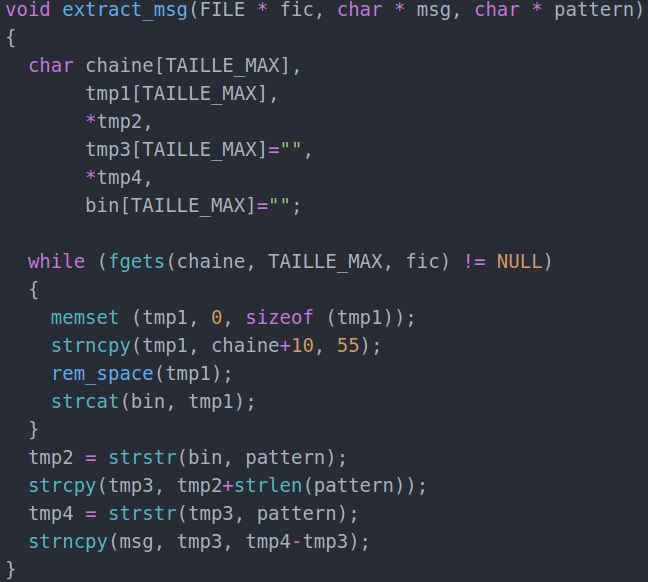
\includegraphics[scale=0.38]{images/extract_message.png}
\end{frame}